\documentclass[twoside]{book}

% Packages required by doxygen
\usepackage{fixltx2e}
\usepackage{calc}
\usepackage{doxygen}
\usepackage[export]{adjustbox} % also loads graphicx
\usepackage{graphicx}
\usepackage[utf8]{inputenc}
\usepackage{makeidx}
\usepackage{multicol}
\usepackage{multirow}
\PassOptionsToPackage{warn}{textcomp}
\usepackage{textcomp}
\usepackage[nointegrals]{wasysym}
\usepackage[table]{xcolor}

% Font selection
\usepackage[T1]{fontenc}
\usepackage[scaled=.90]{helvet}
\usepackage{courier}
\usepackage{amssymb}
\usepackage{sectsty}
\renewcommand{\familydefault}{\sfdefault}
\allsectionsfont{%
  \fontseries{bc}\selectfont%
  \color{darkgray}%
}
\renewcommand{\DoxyLabelFont}{%
  \fontseries{bc}\selectfont%
  \color{darkgray}%
}
\newcommand{\+}{\discretionary{\mbox{\scriptsize$\hookleftarrow$}}{}{}}

% Page & text layout
\usepackage{geometry}
\geometry{%
  a4paper,%
  top=2.5cm,%
  bottom=2.5cm,%
  left=2.5cm,%
  right=2.5cm%
}
\tolerance=750
\hfuzz=15pt
\hbadness=750
\setlength{\emergencystretch}{15pt}
\setlength{\parindent}{0cm}
\setlength{\parskip}{3ex plus 2ex minus 2ex}
\makeatletter
\renewcommand{\paragraph}{%
  \@startsection{paragraph}{4}{0ex}{-1.0ex}{1.0ex}{%
    \normalfont\normalsize\bfseries\SS@parafont%
  }%
}
\renewcommand{\subparagraph}{%
  \@startsection{subparagraph}{5}{0ex}{-1.0ex}{1.0ex}{%
    \normalfont\normalsize\bfseries\SS@subparafont%
  }%
}
\makeatother

% Headers & footers
\usepackage{fancyhdr}
\pagestyle{fancyplain}
\fancyhead[LE]{\fancyplain{}{\bfseries\thepage}}
\fancyhead[CE]{\fancyplain{}{}}
\fancyhead[RE]{\fancyplain{}{\bfseries\leftmark}}
\fancyhead[LO]{\fancyplain{}{\bfseries\rightmark}}
\fancyhead[CO]{\fancyplain{}{}}
\fancyhead[RO]{\fancyplain{}{\bfseries\thepage}}
\fancyfoot[LE]{\fancyplain{}{}}
\fancyfoot[CE]{\fancyplain{}{}}
\fancyfoot[RE]{\fancyplain{}{\bfseries\scriptsize Generated by Doxygen }}
\fancyfoot[LO]{\fancyplain{}{\bfseries\scriptsize Generated by Doxygen }}
\fancyfoot[CO]{\fancyplain{}{}}
\fancyfoot[RO]{\fancyplain{}{}}
\renewcommand{\footrulewidth}{0.4pt}
\renewcommand{\chaptermark}[1]{%
  \markboth{#1}{}%
}
\renewcommand{\sectionmark}[1]{%
  \markright{\thesection\ #1}%
}

% Indices & bibliography
\usepackage{natbib}
\usepackage[titles]{tocloft}
\setcounter{tocdepth}{3}
\setcounter{secnumdepth}{5}
\makeindex

% Hyperlinks (required, but should be loaded last)
\usepackage{ifpdf}
\ifpdf
  \usepackage[pdftex,pagebackref=true]{hyperref}
\else
  \usepackage[ps2pdf,pagebackref=true]{hyperref}
\fi
\hypersetup{%
  colorlinks=true,%
  linkcolor=blue,%
  citecolor=blue,%
  unicode%
}

% Custom commands
\newcommand{\clearemptydoublepage}{%
  \newpage{\pagestyle{empty}\cleardoublepage}%
}

\usepackage{caption}
\captionsetup{labelsep=space,justification=centering,font={bf},singlelinecheck=off,skip=4pt,position=top}

%===== C O N T E N T S =====

\begin{document}

% Titlepage & ToC
\hypersetup{pageanchor=false,
             bookmarksnumbered=true,
             pdfencoding=unicode
            }
\pagenumbering{roman}
\begin{titlepage}
\vspace*{7cm}
\begin{center}%
{\Large Tram Netwerk }\\
\vspace*{1cm}
{\large Generated by Doxygen 1.8.11}\\
\end{center}
\end{titlepage}
\clearemptydoublepage
\tableofcontents
\clearemptydoublepage
\pagenumbering{arabic}
\hypersetup{pageanchor=true}

%--- Begin generated contents ---
\chapter{Class Index}
\section{Class List}
Here are the classes, structs, unions and interfaces with brief descriptions\+:\begin{DoxyCompactList}
\item\contentsline{section}{\hyperlink{classStation}{Station} }{\pageref{classStation}}{}
\end{DoxyCompactList}

\chapter{File Index}
\section{File List}
Here is a list of all documented files with brief descriptions\+:\begin{DoxyCompactList}
\item\contentsline{section}{src/\+Parser/\hyperlink{Parser_8h}{Parser.\+h} \\*Header file for the \hyperlink{classParser}{Parser} Class }{\pageref{Parser_8h}}{}
\item\contentsline{section}{src/\+Passagier/\hyperlink{Passagier_8h}{Passagier.\+h} \\*Header file for the \hyperlink{classPassagier}{Passagier} Class }{\pageref{Passagier_8h}}{}
\item\contentsline{section}{src/\+Spoor/\hyperlink{Spoor_8h}{Spoor.\+h} \\*Header file for the \hyperlink{classSpoor}{Spoor} Class }{\pageref{Spoor_8h}}{}
\item\contentsline{section}{src/\+Station/\hyperlink{Halte_8h}{Halte.\+h} \\*Header file for the \hyperlink{classHalte}{Halte} Class }{\pageref{Halte_8h}}{}
\item\contentsline{section}{src/\+Station/\hyperlink{Metrostation_8h}{Metrostation.\+h} \\*Header file for the \hyperlink{classMetrostation}{Metrostation} Class }{\pageref{Metrostation_8h}}{}
\item\contentsline{section}{src/\+Station/\hyperlink{Station_8h}{Station.\+h} \\*Header file for the \hyperlink{classStation}{Station} Class }{\pageref{Station_8h}}{}
\item\contentsline{section}{src/\+System/\hyperlink{System_8h}{System.\+h} \\*Header file for \hyperlink{classSystem}{System} class }{\pageref{System_8h}}{}
\item\contentsline{section}{src/tinyxml/{\bfseries tinystr.\+h} }{\pageref{tinystr_8h}}{}
\item\contentsline{section}{src/tinyxml/{\bfseries tinyxml.\+h} }{\pageref{tinyxml_8h}}{}
\item\contentsline{section}{src/\+Tram/\hyperlink{Albatros_8h}{Albatros.\+h} \\*Header file for the \hyperlink{classAlbatros}{Albatros} Class }{\pageref{Albatros_8h}}{}
\item\contentsline{section}{src/\+Tram/{\bfseries P\+C\+C.\+h} }{\pageref{PCC_8h}}{}
\item\contentsline{section}{src/\+Tram/\hyperlink{Tram_8h}{Tram.\+h} \\*Header file for the \hyperlink{classPCC}{P\+CC} Class }{\pageref{Tram_8h}}{}
\end{DoxyCompactList}

\chapter{Class Documentation}
\hypertarget{classParser}{}\section{Parser Class Reference}
\label{classParser}\index{Parser@{Parser}}


This Class contains all the functionalities for the \hyperlink{classParser}{Parser} objects.  




{\ttfamily \#include $<$Parser.\+h$>$}

\subsection*{Public Member Functions}
\begin{DoxyCompactItemize}
\item 
\hyperlink{classParser_a12234f6cd36b61af4b50c94a179422c1}{Parser} ()\hypertarget{classParser_a12234f6cd36b61af4b50c94a179422c1}{}\label{classParser_a12234f6cd36b61af4b50c94a179422c1}

\begin{DoxyCompactList}\small\item\em \hyperlink{classParser}{Parser} Default Constructor. \end{DoxyCompactList}\item 
\hyperlink{classSystem}{System} $\ast$ \hyperlink{classParser_addad80574e43b744a82807d0f821d414}{get\+System} () const 
\begin{DoxyCompactList}\small\item\em Returns the \hyperlink{classParser}{Parser} object\textquotesingle{}s \hyperlink{classSystem}{System} Object. \end{DoxyCompactList}\item 
void {\bfseries set\+System} (\hyperlink{classSystem}{System} $\ast$system)\hypertarget{classParser_aaf58c6aafde4e7b889fbaa5d1f3aa6fe}{}\label{classParser_aaf58c6aafde4e7b889fbaa5d1f3aa6fe}

\item 
string \hyperlink{classParser_a36b746dbf631544851e0af2d0e7c6982}{get\+Element} (\hyperlink{classTiXmlElement}{Ti\+Xml\+Element} $\ast$elem)
\begin{DoxyCompactList}\small\item\em Returns the text contained in a \hyperlink{classTiXmlElement}{Ti\+Xml\+Element} Object. \end{DoxyCompactList}\item 
bool \hyperlink{classParser_aa8cdba8032e5d5d87b249be597b196c7}{Xml\+Parser} (string input\+File)
\begin{DoxyCompactList}\small\item\em Returns true if the inputfile is correctly parsed, false if not. \end{DoxyCompactList}\item 
bool \hyperlink{classParser_a8f97eab6905436595f33dc82b8957bbd}{is\+\_\+number} (string s)
\begin{DoxyCompactList}\small\item\em Returns true if the entered string is a number, false if not. \end{DoxyCompactList}\end{DoxyCompactItemize}


\subsection{Detailed Description}
This Class contains all the functionalities for the \hyperlink{classParser}{Parser} objects. 

\begin{DoxyAuthor}{Authors}
Loreas Clonen \& Luuk van Sloun 
\end{DoxyAuthor}


\subsection{Member Function Documentation}
\index{Parser@{Parser}!get\+Element@{get\+Element}}
\index{get\+Element@{get\+Element}!Parser@{Parser}}
\subsubsection[{\texorpdfstring{get\+Element(\+Ti\+Xml\+Element $\ast$elem)}{getElement(TiXmlElement *elem)}}]{\setlength{\rightskip}{0pt plus 5cm}string Parser\+::get\+Element (
\begin{DoxyParamCaption}
\item[{{\bf Ti\+Xml\+Element} $\ast$}]{elem}
\end{DoxyParamCaption}
)}\hypertarget{classParser_a36b746dbf631544851e0af2d0e7c6982}{}\label{classParser_a36b746dbf631544851e0af2d0e7c6982}


Returns the text contained in a \hyperlink{classTiXmlElement}{Ti\+Xml\+Element} Object. 

\begin{DoxyReturn}{Returns}
string 
\end{DoxyReturn}
\index{Parser@{Parser}!get\+System@{get\+System}}
\index{get\+System@{get\+System}!Parser@{Parser}}
\subsubsection[{\texorpdfstring{get\+System() const }{getSystem() const }}]{\setlength{\rightskip}{0pt plus 5cm}{\bf System} $\ast$ Parser\+::get\+System (
\begin{DoxyParamCaption}
{}
\end{DoxyParamCaption}
) const}\hypertarget{classParser_addad80574e43b744a82807d0f821d414}{}\label{classParser_addad80574e43b744a82807d0f821d414}


Returns the \hyperlink{classParser}{Parser} object\textquotesingle{}s \hyperlink{classSystem}{System} Object. 

Sets a new \hyperlink{classParser}{Parser} object\textquotesingle{}s \hyperlink{classSystem}{System} Object.

\begin{DoxyReturn}{Returns}
\hyperlink{classSystem}{System} Pointer
\end{DoxyReturn}

\begin{DoxyParams}{Parameters}
{\em system} & -\/ \hyperlink{classSystem}{System} Pointer \\
\hline
\end{DoxyParams}
\index{Parser@{Parser}!is\+\_\+number@{is\+\_\+number}}
\index{is\+\_\+number@{is\+\_\+number}!Parser@{Parser}}
\subsubsection[{\texorpdfstring{is\+\_\+number(string s)}{is_number(string s)}}]{\setlength{\rightskip}{0pt plus 5cm}bool Parser\+::is\+\_\+number (
\begin{DoxyParamCaption}
\item[{string}]{s}
\end{DoxyParamCaption}
)}\hypertarget{classParser_a8f97eab6905436595f33dc82b8957bbd}{}\label{classParser_a8f97eab6905436595f33dc82b8957bbd}


Returns true if the entered string is a number, false if not. 

\begin{DoxyReturn}{Returns}
boolean 
\end{DoxyReturn}
\index{Parser@{Parser}!Xml\+Parser@{Xml\+Parser}}
\index{Xml\+Parser@{Xml\+Parser}!Parser@{Parser}}
\subsubsection[{\texorpdfstring{Xml\+Parser(string input\+File)}{XmlParser(string inputFile)}}]{\setlength{\rightskip}{0pt plus 5cm}bool Parser\+::\+Xml\+Parser (
\begin{DoxyParamCaption}
\item[{string}]{input\+File}
\end{DoxyParamCaption}
)}\hypertarget{classParser_aa8cdba8032e5d5d87b249be597b196c7}{}\label{classParser_aa8cdba8032e5d5d87b249be597b196c7}


Returns true if the inputfile is correctly parsed, false if not. 

\begin{DoxyReturn}{Returns}
boolean 
\end{DoxyReturn}


The documentation for this class was generated from the following files\+:\begin{DoxyCompactItemize}
\item 
src/\+Parser/\hyperlink{Parser_8h}{Parser.\+h}\item 
src/\+Parser/Parser.\+cpp\end{DoxyCompactItemize}

\hypertarget{classPassagier}{}\section{Passagier Class Reference}
\label{classPassagier}\index{Passagier@{Passagier}}


This Class contains all the functionalities for the \hyperlink{classPassagier}{Passagier} objects.  




{\ttfamily \#include $<$Passagier.\+h$>$}

\subsection*{Public Member Functions}
\begin{DoxyCompactItemize}
\item 
\hyperlink{classPassagier_a1a2bc82f5780448cd2a9a47d08cc824f}{Passagier} ()\hypertarget{classPassagier_a1a2bc82f5780448cd2a9a47d08cc824f}{}\label{classPassagier_a1a2bc82f5780448cd2a9a47d08cc824f}

\begin{DoxyCompactList}\small\item\em Passenger Default Constructor. \end{DoxyCompactList}\item 
bool \hyperlink{classPassagier_ae271ce7875b2a7d17704e204ce9d8568}{properly\+Initialized} ()
\begin{DoxyCompactList}\small\item\em Returns true if properly initialized, false if not. \end{DoxyCompactList}\item 
string \hyperlink{classPassagier_aa9a9b53d417979551b0cb30fb0fdd232}{get\+Naam} ()
\begin{DoxyCompactList}\small\item\em Returns the \hyperlink{classStation}{Station} object\textquotesingle{}s name. \end{DoxyCompactList}\item 
void \hyperlink{classPassagier_a8d7a04358b35de18f378d048610e9aff}{set\+Naam} (string naam)
\begin{DoxyCompactList}\small\item\em Sets a new Passenger object\textquotesingle{}s name. \end{DoxyCompactList}\item 
string \hyperlink{classPassagier_a41e0870bb942364181aa17e2c9c7ca6c}{get\+Begin\+Station} ()
\begin{DoxyCompactList}\small\item\em Returns the Passenger object\textquotesingle{}s Starting \hyperlink{classStation}{Station}. \end{DoxyCompactList}\item 
void \hyperlink{classPassagier_afc4826ff4dacbbe15f15f6e8ef338ff0}{set\+Begin\+Station} (string begin\+Station)
\begin{DoxyCompactList}\small\item\em Sets a new Passenger object\textquotesingle{}s Starting \hyperlink{classStation}{Station}. \end{DoxyCompactList}\item 
string \hyperlink{classPassagier_a721949463e02e122567c9967786a8a38}{get\+Eind\+Station} ()
\begin{DoxyCompactList}\small\item\em Returns the Passenger object\textquotesingle{}s End \hyperlink{classStation}{Station}. \end{DoxyCompactList}\item 
void \hyperlink{classPassagier_a93606f0982849fc1838b5e16ab5f1b12}{set\+Eind\+Station} (string eind\+Station)
\begin{DoxyCompactList}\small\item\em Sets a new Passenger object\textquotesingle{}s End \hyperlink{classStation}{Station}. \end{DoxyCompactList}\item 
int \hyperlink{classPassagier_a1fd825eaa3db5b68cc24ca297e45d198}{get\+Hoeveelheid} ()
\begin{DoxyCompactList}\small\item\em Returns the Passenger object\textquotesingle{}s amount. \end{DoxyCompactList}\item 
void \hyperlink{classPassagier_adf498b0e24ef821f30e479591da7a3d3}{set\+Hoeveelheid} (int hoeveelheid)
\begin{DoxyCompactList}\small\item\em Sets a new Passenger object\textquotesingle{}s amount. \end{DoxyCompactList}\end{DoxyCompactItemize}


\subsection{Detailed Description}
This Class contains all the functionalities for the \hyperlink{classPassagier}{Passagier} objects. 

\begin{DoxyAuthor}{Authors}
Loreas Clonen \& Luuk van Sloun 
\end{DoxyAuthor}


\subsection{Member Function Documentation}
\index{Passagier@{Passagier}!get\+Begin\+Station@{get\+Begin\+Station}}
\index{get\+Begin\+Station@{get\+Begin\+Station}!Passagier@{Passagier}}
\subsubsection[{\texorpdfstring{get\+Begin\+Station()}{getBeginStation()}}]{\setlength{\rightskip}{0pt plus 5cm}string Passagier\+::get\+Begin\+Station (
\begin{DoxyParamCaption}
{}
\end{DoxyParamCaption}
)}\hypertarget{classPassagier_a41e0870bb942364181aa17e2c9c7ca6c}{}\label{classPassagier_a41e0870bb942364181aa17e2c9c7ca6c}


Returns the Passenger object\textquotesingle{}s Starting \hyperlink{classStation}{Station}. 

\begin{DoxyReturn}{Returns}
string 
\end{DoxyReturn}
\index{Passagier@{Passagier}!get\+Eind\+Station@{get\+Eind\+Station}}
\index{get\+Eind\+Station@{get\+Eind\+Station}!Passagier@{Passagier}}
\subsubsection[{\texorpdfstring{get\+Eind\+Station()}{getEindStation()}}]{\setlength{\rightskip}{0pt plus 5cm}string Passagier\+::get\+Eind\+Station (
\begin{DoxyParamCaption}
{}
\end{DoxyParamCaption}
)}\hypertarget{classPassagier_a721949463e02e122567c9967786a8a38}{}\label{classPassagier_a721949463e02e122567c9967786a8a38}


Returns the Passenger object\textquotesingle{}s End \hyperlink{classStation}{Station}. 

\begin{DoxyReturn}{Returns}
string 
\end{DoxyReturn}
\index{Passagier@{Passagier}!get\+Hoeveelheid@{get\+Hoeveelheid}}
\index{get\+Hoeveelheid@{get\+Hoeveelheid}!Passagier@{Passagier}}
\subsubsection[{\texorpdfstring{get\+Hoeveelheid()}{getHoeveelheid()}}]{\setlength{\rightskip}{0pt plus 5cm}string Passagier\+::get\+Hoeveelheid (
\begin{DoxyParamCaption}
{}
\end{DoxyParamCaption}
)}\hypertarget{classPassagier_a1fd825eaa3db5b68cc24ca297e45d198}{}\label{classPassagier_a1fd825eaa3db5b68cc24ca297e45d198}


Returns the Passenger object\textquotesingle{}s amount. 

\begin{DoxyReturn}{Returns}
integer 
\end{DoxyReturn}
\index{Passagier@{Passagier}!get\+Naam@{get\+Naam}}
\index{get\+Naam@{get\+Naam}!Passagier@{Passagier}}
\subsubsection[{\texorpdfstring{get\+Naam()}{getNaam()}}]{\setlength{\rightskip}{0pt plus 5cm}string Passagier\+::get\+Naam (
\begin{DoxyParamCaption}
{}
\end{DoxyParamCaption}
)}\hypertarget{classPassagier_aa9a9b53d417979551b0cb30fb0fdd232}{}\label{classPassagier_aa9a9b53d417979551b0cb30fb0fdd232}


Returns the \hyperlink{classStation}{Station} object\textquotesingle{}s name. 

\begin{DoxyReturn}{Returns}
string 
\end{DoxyReturn}
\index{Passagier@{Passagier}!properly\+Initialized@{properly\+Initialized}}
\index{properly\+Initialized@{properly\+Initialized}!Passagier@{Passagier}}
\subsubsection[{\texorpdfstring{properly\+Initialized()}{properlyInitialized()}}]{\setlength{\rightskip}{0pt plus 5cm}bool Passagier\+::properly\+Initialized (
\begin{DoxyParamCaption}
{}
\end{DoxyParamCaption}
)}\hypertarget{classPassagier_ae271ce7875b2a7d17704e204ce9d8568}{}\label{classPassagier_ae271ce7875b2a7d17704e204ce9d8568}


Returns true if properly initialized, false if not. 

\begin{DoxyReturn}{Returns}
boolean 
\end{DoxyReturn}
\index{Passagier@{Passagier}!set\+Begin\+Station@{set\+Begin\+Station}}
\index{set\+Begin\+Station@{set\+Begin\+Station}!Passagier@{Passagier}}
\subsubsection[{\texorpdfstring{set\+Begin\+Station(string begin\+Station)}{setBeginStation(string beginStation)}}]{\setlength{\rightskip}{0pt plus 5cm}void Passagier\+::set\+Begin\+Station (
\begin{DoxyParamCaption}
\item[{string}]{begin\+Station}
\end{DoxyParamCaption}
)}\hypertarget{classPassagier_afc4826ff4dacbbe15f15f6e8ef338ff0}{}\label{classPassagier_afc4826ff4dacbbe15f15f6e8ef338ff0}


Sets a new Passenger object\textquotesingle{}s Starting \hyperlink{classStation}{Station}. 


\begin{DoxyParams}{Parameters}
{\em begin\+Station} & -\/ string \\
\hline
\end{DoxyParams}
\index{Passagier@{Passagier}!set\+Eind\+Station@{set\+Eind\+Station}}
\index{set\+Eind\+Station@{set\+Eind\+Station}!Passagier@{Passagier}}
\subsubsection[{\texorpdfstring{set\+Eind\+Station(string eind\+Station)}{setEindStation(string eindStation)}}]{\setlength{\rightskip}{0pt plus 5cm}void Passagier\+::set\+Eind\+Station (
\begin{DoxyParamCaption}
\item[{string}]{eind\+Station}
\end{DoxyParamCaption}
)}\hypertarget{classPassagier_a93606f0982849fc1838b5e16ab5f1b12}{}\label{classPassagier_a93606f0982849fc1838b5e16ab5f1b12}


Sets a new Passenger object\textquotesingle{}s End \hyperlink{classStation}{Station}. 


\begin{DoxyParams}{Parameters}
{\em eind\+Station} & -\/ string \\
\hline
\end{DoxyParams}
\index{Passagier@{Passagier}!set\+Hoeveelheid@{set\+Hoeveelheid}}
\index{set\+Hoeveelheid@{set\+Hoeveelheid}!Passagier@{Passagier}}
\subsubsection[{\texorpdfstring{set\+Hoeveelheid(int hoeveelheid)}{setHoeveelheid(int hoeveelheid)}}]{\setlength{\rightskip}{0pt plus 5cm}void Passagier\+::set\+Hoeveelheid (
\begin{DoxyParamCaption}
\item[{int}]{hoeveelheid}
\end{DoxyParamCaption}
)}\hypertarget{classPassagier_adf498b0e24ef821f30e479591da7a3d3}{}\label{classPassagier_adf498b0e24ef821f30e479591da7a3d3}


Sets a new Passenger object\textquotesingle{}s amount. 


\begin{DoxyParams}{Parameters}
{\em hoeveelheid} & -\/ integer \\
\hline
\end{DoxyParams}
\index{Passagier@{Passagier}!set\+Naam@{set\+Naam}}
\index{set\+Naam@{set\+Naam}!Passagier@{Passagier}}
\subsubsection[{\texorpdfstring{set\+Naam(string naam)}{setNaam(string naam)}}]{\setlength{\rightskip}{0pt plus 5cm}void Passagier\+::set\+Naam (
\begin{DoxyParamCaption}
\item[{string}]{naam}
\end{DoxyParamCaption}
)}\hypertarget{classPassagier_a8d7a04358b35de18f378d048610e9aff}{}\label{classPassagier_a8d7a04358b35de18f378d048610e9aff}


Sets a new Passenger object\textquotesingle{}s name. 


\begin{DoxyParams}{Parameters}
{\em naam} & -\/ string \\
\hline
\end{DoxyParams}


The documentation for this class was generated from the following files\+:\begin{DoxyCompactItemize}
\item 
src/\hyperlink{Passagier_8h}{Passagier.\+h}\item 
src/Passagier.\+cpp\end{DoxyCompactItemize}

\hypertarget{classSpoor}{}\section{Spoor Class Reference}
\label{classSpoor}\index{Spoor@{Spoor}}


This Class contains all the functionalities for the \hyperlink{classSpoor}{Spoor} objects.  




{\ttfamily \#include $<$Spoor.\+h$>$}

\subsection*{Public Member Functions}
\begin{DoxyCompactItemize}
\item 
\hyperlink{classSpoor_a64778a4094d2d9cd3a08cbbef5a11787}{Spoor} ()
\begin{DoxyCompactList}\small\item\em \hyperlink{classSpoor}{Spoor} Default Constructor. \end{DoxyCompactList}\item 
bool \hyperlink{classSpoor_a31982084b33e5946f1e15844b084f62f}{properly\+Initialized} ()
\begin{DoxyCompactList}\small\item\em Returns true if properly initialized, false if not. \end{DoxyCompactList}\item 
int \hyperlink{classSpoor_a17c71f600581bc91b85c92d6628d14c5}{get\+Spoor\+Nr} ()
\begin{DoxyCompactList}\small\item\em Returns the \hyperlink{classSpoor}{Spoor} object\textquotesingle{}s Track Number. \end{DoxyCompactList}\item 
void \hyperlink{classSpoor_af0c947d95aafed41f4fa3c5ec96d2e3c}{set\+Spoor\+Nr} (int spoor\+Nr)
\begin{DoxyCompactList}\small\item\em Sets a new \hyperlink{classSpoor}{Spoor} object\textquotesingle{}s Track Number. \end{DoxyCompactList}\item 
string \hyperlink{classSpoor_af72fa63d73e10bb5d0bb0e15958260d5}{get\+Volgende} ()
\begin{DoxyCompactList}\small\item\em Returns the \hyperlink{classStation}{Station} object\textquotesingle{}s Next \hyperlink{classStation}{Station}. \end{DoxyCompactList}\item 
void \hyperlink{classSpoor_a3f372480028541bed83821716b90da58}{set\+Volgende} (string volgende)
\begin{DoxyCompactList}\small\item\em Sets a new \hyperlink{classSpoor}{Spoor} object\textquotesingle{}s Next \hyperlink{classStation}{Station}. \end{DoxyCompactList}\item 
string \hyperlink{classSpoor_a4c9a290c147e08e5734c662c73b9793c}{get\+Vorige} ()
\begin{DoxyCompactList}\small\item\em Returns the \hyperlink{classStation}{Station} object\textquotesingle{}s Previous \hyperlink{classStation}{Station}. \end{DoxyCompactList}\item 
void \hyperlink{classSpoor_a7f6d776cfd20986866011f1a42a6c762}{set\+Vorige} (string vorige)
\begin{DoxyCompactList}\small\item\em Sets a new \hyperlink{classSpoor}{Spoor} object\textquotesingle{}s Previous \hyperlink{classStation}{Station}. \end{DoxyCompactList}\end{DoxyCompactItemize}


\subsection{Detailed Description}
This Class contains all the functionalities for the \hyperlink{classSpoor}{Spoor} objects. 

\begin{DoxyAuthor}{Authors}
Loreas Clonen \& Luuk van Sloun 
\end{DoxyAuthor}


\subsection{Constructor \& Destructor Documentation}
\index{Spoor@{Spoor}!Spoor@{Spoor}}
\index{Spoor@{Spoor}!Spoor@{Spoor}}
\subsubsection[{\texorpdfstring{Spoor()}{Spoor()}}]{\setlength{\rightskip}{0pt plus 5cm}Spoor\+::\+Spoor (
\begin{DoxyParamCaption}
{}
\end{DoxyParamCaption}
)}\hypertarget{classSpoor_a64778a4094d2d9cd3a08cbbef5a11787}{}\label{classSpoor_a64778a4094d2d9cd3a08cbbef5a11787}


\hyperlink{classSpoor}{Spoor} Default Constructor. 

\begin{DoxyPostcond}{Postcondition}
A new \hyperlink{classSpoor}{Spoor} Object has been created 
\end{DoxyPostcond}


\subsection{Member Function Documentation}
\index{Spoor@{Spoor}!get\+Spoor\+Nr@{get\+Spoor\+Nr}}
\index{get\+Spoor\+Nr@{get\+Spoor\+Nr}!Spoor@{Spoor}}
\subsubsection[{\texorpdfstring{get\+Spoor\+Nr()}{getSpoorNr()}}]{\setlength{\rightskip}{0pt plus 5cm}int Spoor\+::get\+Spoor\+Nr (
\begin{DoxyParamCaption}
{}
\end{DoxyParamCaption}
)}\hypertarget{classSpoor_a17c71f600581bc91b85c92d6628d14c5}{}\label{classSpoor_a17c71f600581bc91b85c92d6628d14c5}


Returns the \hyperlink{classSpoor}{Spoor} object\textquotesingle{}s Track Number. 

\begin{DoxyPrecond}{Precondition}
The \hyperlink{classSpoor}{Spoor} Object has been properly initialized 

The \hyperlink{classSpoor}{Spoor} Object has a non-\/empty member variable spoor\+Nr 
\end{DoxyPrecond}
\begin{DoxyReturn}{Returns}
integer 
\end{DoxyReturn}
\index{Spoor@{Spoor}!get\+Volgende@{get\+Volgende}}
\index{get\+Volgende@{get\+Volgende}!Spoor@{Spoor}}
\subsubsection[{\texorpdfstring{get\+Volgende()}{getVolgende()}}]{\setlength{\rightskip}{0pt plus 5cm}string Spoor\+::get\+Volgende (
\begin{DoxyParamCaption}
{}
\end{DoxyParamCaption}
)}\hypertarget{classSpoor_af72fa63d73e10bb5d0bb0e15958260d5}{}\label{classSpoor_af72fa63d73e10bb5d0bb0e15958260d5}


Returns the \hyperlink{classStation}{Station} object\textquotesingle{}s Next \hyperlink{classStation}{Station}. 

\begin{DoxyPrecond}{Precondition}
The \hyperlink{classSpoor}{Spoor} Object has been properly initialized 

The \hyperlink{classSpoor}{Spoor} Object has a non-\/empty member variable volgende 
\end{DoxyPrecond}
\begin{DoxyReturn}{Returns}
string 
\end{DoxyReturn}
\index{Spoor@{Spoor}!get\+Vorige@{get\+Vorige}}
\index{get\+Vorige@{get\+Vorige}!Spoor@{Spoor}}
\subsubsection[{\texorpdfstring{get\+Vorige()}{getVorige()}}]{\setlength{\rightskip}{0pt plus 5cm}string Spoor\+::get\+Vorige (
\begin{DoxyParamCaption}
{}
\end{DoxyParamCaption}
)}\hypertarget{classSpoor_a4c9a290c147e08e5734c662c73b9793c}{}\label{classSpoor_a4c9a290c147e08e5734c662c73b9793c}


Returns the \hyperlink{classStation}{Station} object\textquotesingle{}s Previous \hyperlink{classStation}{Station}. 

\begin{DoxyPrecond}{Precondition}
The \hyperlink{classSpoor}{Spoor} Object has been properly initialized 

The \hyperlink{classSpoor}{Spoor} Object has a non-\/empty member variable vorige 
\end{DoxyPrecond}
\begin{DoxyReturn}{Returns}
string 
\end{DoxyReturn}
\index{Spoor@{Spoor}!properly\+Initialized@{properly\+Initialized}}
\index{properly\+Initialized@{properly\+Initialized}!Spoor@{Spoor}}
\subsubsection[{\texorpdfstring{properly\+Initialized()}{properlyInitialized()}}]{\setlength{\rightskip}{0pt plus 5cm}bool Spoor\+::properly\+Initialized (
\begin{DoxyParamCaption}
{}
\end{DoxyParamCaption}
)}\hypertarget{classSpoor_a31982084b33e5946f1e15844b084f62f}{}\label{classSpoor_a31982084b33e5946f1e15844b084f62f}


Returns true if properly initialized, false if not. 

\begin{DoxyReturn}{Returns}
boolean 
\end{DoxyReturn}
\index{Spoor@{Spoor}!set\+Spoor\+Nr@{set\+Spoor\+Nr}}
\index{set\+Spoor\+Nr@{set\+Spoor\+Nr}!Spoor@{Spoor}}
\subsubsection[{\texorpdfstring{set\+Spoor\+Nr(int spoor\+Nr)}{setSpoorNr(int spoorNr)}}]{\setlength{\rightskip}{0pt plus 5cm}int Spoor\+::set\+Spoor\+Nr (
\begin{DoxyParamCaption}
\item[{int}]{spoor\+Nr}
\end{DoxyParamCaption}
)}\hypertarget{classSpoor_af0c947d95aafed41f4fa3c5ec96d2e3c}{}\label{classSpoor_af0c947d95aafed41f4fa3c5ec96d2e3c}


Sets a new \hyperlink{classSpoor}{Spoor} object\textquotesingle{}s Track Number. 


\begin{DoxyParams}{Parameters}
{\em spoor\+Nr} & -\/ integer \\
\hline
\end{DoxyParams}
\begin{DoxyPrecond}{Precondition}
The \hyperlink{classSpoor}{Spoor} Object has been properly initialized 

spoor\+Nr is a positive integer 
\end{DoxyPrecond}
\begin{DoxyPostcond}{Postcondition}
The \hyperlink{classSpoor}{Spoor} Object\textquotesingle{}s Track Number is equal to variable spoor\+Nr 
\end{DoxyPostcond}
\index{Spoor@{Spoor}!set\+Volgende@{set\+Volgende}}
\index{set\+Volgende@{set\+Volgende}!Spoor@{Spoor}}
\subsubsection[{\texorpdfstring{set\+Volgende(string volgende)}{setVolgende(string volgende)}}]{\setlength{\rightskip}{0pt plus 5cm}void Spoor\+::set\+Volgende (
\begin{DoxyParamCaption}
\item[{string}]{volgende}
\end{DoxyParamCaption}
)}\hypertarget{classSpoor_a3f372480028541bed83821716b90da58}{}\label{classSpoor_a3f372480028541bed83821716b90da58}


Sets a new \hyperlink{classSpoor}{Spoor} object\textquotesingle{}s Next \hyperlink{classStation}{Station}. 


\begin{DoxyParams}{Parameters}
{\em volgende} & -\/ string \\
\hline
\end{DoxyParams}
\begin{DoxyPrecond}{Precondition}
The \hyperlink{classSpoor}{Spoor} Object has been properly initialized 

volgende is a non-\/empty string 
\end{DoxyPrecond}
\begin{DoxyPostcond}{Postcondition}
The \hyperlink{classSpoor}{Spoor} Object\textquotesingle{}s Next \hyperlink{classStation}{Station} is equal to variable volgende 
\end{DoxyPostcond}
\index{Spoor@{Spoor}!set\+Vorige@{set\+Vorige}}
\index{set\+Vorige@{set\+Vorige}!Spoor@{Spoor}}
\subsubsection[{\texorpdfstring{set\+Vorige(string vorige)}{setVorige(string vorige)}}]{\setlength{\rightskip}{0pt plus 5cm}void Spoor\+::set\+Vorige (
\begin{DoxyParamCaption}
\item[{string}]{vorige}
\end{DoxyParamCaption}
)}\hypertarget{classSpoor_a7f6d776cfd20986866011f1a42a6c762}{}\label{classSpoor_a7f6d776cfd20986866011f1a42a6c762}


Sets a new \hyperlink{classSpoor}{Spoor} object\textquotesingle{}s Previous \hyperlink{classStation}{Station}. 


\begin{DoxyParams}{Parameters}
{\em vorige} & -\/ string \\
\hline
\end{DoxyParams}
\begin{DoxyPrecond}{Precondition}
The \hyperlink{classSpoor}{Spoor} Object has been properly initialized 

vorige is a non-\/empty string 
\end{DoxyPrecond}
\begin{DoxyPostcond}{Postcondition}
The \hyperlink{classSpoor}{Spoor} Object\textquotesingle{}s Next \hyperlink{classStation}{Station} is equal to variable vorige 
\end{DoxyPostcond}


The documentation for this class was generated from the following files\+:\begin{DoxyCompactItemize}
\item 
src/\+Spoor/\hyperlink{Spoor_8h}{Spoor.\+h}\item 
src/\+Spoor/Spoor.\+cpp\end{DoxyCompactItemize}

\hypertarget{classStation}{}\section{Station Class Reference}
\label{classStation}\index{Station@{Station}}


This Class contains all the functionalities for the \hyperlink{classStation}{Station} objects.  




{\ttfamily \#include $<$Station.\+h$>$}

\subsection*{Public Member Functions}
\begin{DoxyCompactItemize}
\item 
\hyperlink{classStation_a73d335726aad1d844d81cda6d9fd74e6}{Station} ()\hypertarget{classStation_a73d335726aad1d844d81cda6d9fd74e6}{}\label{classStation_a73d335726aad1d844d81cda6d9fd74e6}

\begin{DoxyCompactList}\small\item\em \hyperlink{classStation}{Station} Default Constructor. \end{DoxyCompactList}\item 
string \hyperlink{classStation_a7db91849f0d5bab0a4ac0aa4967721cf}{get\+Naam} ()
\begin{DoxyCompactList}\small\item\em Returns the \hyperlink{classStation}{Station} object\textquotesingle{}s name. \end{DoxyCompactList}\item 
void \hyperlink{classStation_a9838301eaa0d45561877bcebc19a663c}{set\+Naam} (string naam)
\begin{DoxyCompactList}\small\item\em Sets a new \hyperlink{classStation}{Station} object\textquotesingle{}s name. \end{DoxyCompactList}\item 
bool \hyperlink{classStation_aab182a50a2992afe0df4412f7de4b73d}{properly\+Initialized} ()
\begin{DoxyCompactList}\small\item\em Returns true if properly initialized, false if not. \end{DoxyCompactList}\item 
string \hyperlink{classStation_aac519858a1ac53608d24d78e4b9231ab}{get\+Type} ()
\begin{DoxyCompactList}\small\item\em Returns the \hyperlink{classStation}{Station} object\textquotesingle{}s type. \end{DoxyCompactList}\item 
void \hyperlink{classStation_a1a38a1c6db22cfda3c5885281252a3b9}{set\+Type} (string type)
\begin{DoxyCompactList}\small\item\em Sets a new \hyperlink{classStation}{Station} object\textquotesingle{}s type. \end{DoxyCompactList}\item 
void \hyperlink{classStation_a9584a65058bdf75254e3a2d79ddcdba1}{add\+Passagier} (string \hyperlink{classPassagier}{Passagier})
\begin{DoxyCompactList}\small\item\em Adds a Passenger to the \hyperlink{classStation}{Station} object\textquotesingle{}s Passenger set. \end{DoxyCompactList}\item 
void \hyperlink{classStation_aa250b3ba3e62c3d433b4c29f6cca38d4}{remove\+Passagier} (string \hyperlink{classPassagier}{Passagier})
\begin{DoxyCompactList}\small\item\em Removes a Passenger from the \hyperlink{classStation}{Station} object\textquotesingle{}s Passenger set. \end{DoxyCompactList}\item 
set$<$ string $>$ \hyperlink{classStation_a3c25e627a9036778a4d6d08ca1454aa6}{get\+Passagier} ()
\begin{DoxyCompactList}\small\item\em Returns the \hyperlink{classStation}{Station} object\textquotesingle{}s Passenger set. \end{DoxyCompactList}\item 
map$<$ int, \hyperlink{classSpoor}{Spoor} $\ast$ $>$ \hyperlink{classStation_a8ee617b13d4d67d0d3d1384d6d33226f}{get\+Sporen} ()
\begin{DoxyCompactList}\small\item\em Returns the \hyperlink{classStation}{Station} object\textquotesingle{}s Tracks map. \end{DoxyCompactList}\item 
void \hyperlink{classStation_a55911b5e0a355f085afd75391827729f}{add\+Spoor} (\hyperlink{classSpoor}{Spoor} $\ast$spoor, int spoor\+Nr)
\begin{DoxyCompactList}\small\item\em Adds a new \hyperlink{classStation}{Station} Track to the Tracks map. \end{DoxyCompactList}\item 
virtual string {\bfseries type\+String} ()\hypertarget{classStation_ad83c424982c3e8e85d446593cc833141}{}\label{classStation_ad83c424982c3e8e85d446593cc833141}

\item 
void {\bfseries set\+Sporen} (map$<$ int, \hyperlink{classSpoor}{Spoor} $\ast$ $>$ sporen)\hypertarget{classStation_a036804467eb7a7c3bf51a90b4ee57eee}{}\label{classStation_a036804467eb7a7c3bf51a90b4ee57eee}

\item 
virtual bool {\bfseries is\+Metrostation} ()\hypertarget{classStation_a6c9833b35ffe26df4a0b163c9186be07}{}\label{classStation_a6c9833b35ffe26df4a0b163c9186be07}

\end{DoxyCompactItemize}


\subsection{Detailed Description}
This Class contains all the functionalities for the \hyperlink{classStation}{Station} objects. 

\begin{DoxyAuthor}{Authors}
Loreas Clonen \& Luuk van Sloun 
\end{DoxyAuthor}


\subsection{Member Function Documentation}
\index{Station@{Station}!add\+Passagier@{add\+Passagier}}
\index{add\+Passagier@{add\+Passagier}!Station@{Station}}
\subsubsection[{\texorpdfstring{add\+Passagier(string Passagier)}{addPassagier(string Passagier)}}]{\setlength{\rightskip}{0pt plus 5cm}void Station\+::add\+Passagier (
\begin{DoxyParamCaption}
\item[{string}]{Passagier}
\end{DoxyParamCaption}
)}\hypertarget{classStation_a9584a65058bdf75254e3a2d79ddcdba1}{}\label{classStation_a9584a65058bdf75254e3a2d79ddcdba1}


Adds a Passenger to the \hyperlink{classStation}{Station} object\textquotesingle{}s Passenger set. 


\begin{DoxyParams}{Parameters}
{\em \hyperlink{classPassagier}{Passagier}} & -\/ string \\
\hline
\end{DoxyParams}
\index{Station@{Station}!add\+Spoor@{add\+Spoor}}
\index{add\+Spoor@{add\+Spoor}!Station@{Station}}
\subsubsection[{\texorpdfstring{add\+Spoor(\+Spoor $\ast$spoor, int spoor\+Nr)}{addSpoor(Spoor *spoor, int spoorNr)}}]{\setlength{\rightskip}{0pt plus 5cm}void Station\+::add\+Spoor (
\begin{DoxyParamCaption}
\item[{{\bf Spoor} $\ast$}]{spoor, }
\item[{int}]{spoor\+Nr}
\end{DoxyParamCaption}
)}\hypertarget{classStation_a55911b5e0a355f085afd75391827729f}{}\label{classStation_a55911b5e0a355f085afd75391827729f}


Adds a new \hyperlink{classStation}{Station} Track to the Tracks map. 


\begin{DoxyParams}{Parameters}
{\em spoor} & -\/ \hyperlink{classSpoor}{Spoor} Pointer \\
\hline
{\em spoor\+Nr} & -\/ integer \\
\hline
\end{DoxyParams}
\index{Station@{Station}!get\+Naam@{get\+Naam}}
\index{get\+Naam@{get\+Naam}!Station@{Station}}
\subsubsection[{\texorpdfstring{get\+Naam()}{getNaam()}}]{\setlength{\rightskip}{0pt plus 5cm}string Station\+::get\+Naam (
\begin{DoxyParamCaption}
{}
\end{DoxyParamCaption}
)}\hypertarget{classStation_a7db91849f0d5bab0a4ac0aa4967721cf}{}\label{classStation_a7db91849f0d5bab0a4ac0aa4967721cf}


Returns the \hyperlink{classStation}{Station} object\textquotesingle{}s name. 

\begin{DoxyReturn}{Returns}
string 
\end{DoxyReturn}
\index{Station@{Station}!get\+Passagier@{get\+Passagier}}
\index{get\+Passagier@{get\+Passagier}!Station@{Station}}
\subsubsection[{\texorpdfstring{get\+Passagier()}{getPassagier()}}]{\setlength{\rightskip}{0pt plus 5cm}set$<$ string $>$ Station\+::get\+Passagier (
\begin{DoxyParamCaption}
{}
\end{DoxyParamCaption}
)}\hypertarget{classStation_a3c25e627a9036778a4d6d08ca1454aa6}{}\label{classStation_a3c25e627a9036778a4d6d08ca1454aa6}


Returns the \hyperlink{classStation}{Station} object\textquotesingle{}s Passenger set. 

\begin{DoxyReturn}{Returns}
passagier -\/ set 
\end{DoxyReturn}
\index{Station@{Station}!get\+Sporen@{get\+Sporen}}
\index{get\+Sporen@{get\+Sporen}!Station@{Station}}
\subsubsection[{\texorpdfstring{get\+Sporen()}{getSporen()}}]{\setlength{\rightskip}{0pt plus 5cm}map$<$ int, {\bf Spoor} $\ast$ $>$ Station\+::get\+Sporen (
\begin{DoxyParamCaption}
{}
\end{DoxyParamCaption}
)}\hypertarget{classStation_a8ee617b13d4d67d0d3d1384d6d33226f}{}\label{classStation_a8ee617b13d4d67d0d3d1384d6d33226f}


Returns the \hyperlink{classStation}{Station} object\textquotesingle{}s Tracks map. 

\begin{DoxyReturn}{Returns}
sporen -\/ map 
\end{DoxyReturn}
\index{Station@{Station}!get\+Type@{get\+Type}}
\index{get\+Type@{get\+Type}!Station@{Station}}
\subsubsection[{\texorpdfstring{get\+Type()}{getType()}}]{\setlength{\rightskip}{0pt plus 5cm}string Station\+::get\+Type (
\begin{DoxyParamCaption}
{}
\end{DoxyParamCaption}
)}\hypertarget{classStation_aac519858a1ac53608d24d78e4b9231ab}{}\label{classStation_aac519858a1ac53608d24d78e4b9231ab}


Returns the \hyperlink{classStation}{Station} object\textquotesingle{}s type. 

\begin{DoxyReturn}{Returns}
string 
\end{DoxyReturn}
\index{Station@{Station}!properly\+Initialized@{properly\+Initialized}}
\index{properly\+Initialized@{properly\+Initialized}!Station@{Station}}
\subsubsection[{\texorpdfstring{properly\+Initialized()}{properlyInitialized()}}]{\setlength{\rightskip}{0pt plus 5cm}bool Station\+::properly\+Initialized (
\begin{DoxyParamCaption}
{}
\end{DoxyParamCaption}
)}\hypertarget{classStation_aab182a50a2992afe0df4412f7de4b73d}{}\label{classStation_aab182a50a2992afe0df4412f7de4b73d}


Returns true if properly initialized, false if not. 

\begin{DoxyReturn}{Returns}
boolean 
\end{DoxyReturn}
\index{Station@{Station}!remove\+Passagier@{remove\+Passagier}}
\index{remove\+Passagier@{remove\+Passagier}!Station@{Station}}
\subsubsection[{\texorpdfstring{remove\+Passagier(string Passagier)}{removePassagier(string Passagier)}}]{\setlength{\rightskip}{0pt plus 5cm}void Station\+::remove\+Passagier (
\begin{DoxyParamCaption}
\item[{string}]{Passagier}
\end{DoxyParamCaption}
)}\hypertarget{classStation_aa250b3ba3e62c3d433b4c29f6cca38d4}{}\label{classStation_aa250b3ba3e62c3d433b4c29f6cca38d4}


Removes a Passenger from the \hyperlink{classStation}{Station} object\textquotesingle{}s Passenger set. 


\begin{DoxyParams}{Parameters}
{\em \hyperlink{classPassagier}{Passagier}} & -\/ string \\
\hline
\end{DoxyParams}
\index{Station@{Station}!set\+Naam@{set\+Naam}}
\index{set\+Naam@{set\+Naam}!Station@{Station}}
\subsubsection[{\texorpdfstring{set\+Naam(string naam)}{setNaam(string naam)}}]{\setlength{\rightskip}{0pt plus 5cm}void Station\+::set\+Naam (
\begin{DoxyParamCaption}
\item[{string}]{naam}
\end{DoxyParamCaption}
)}\hypertarget{classStation_a9838301eaa0d45561877bcebc19a663c}{}\label{classStation_a9838301eaa0d45561877bcebc19a663c}


Sets a new \hyperlink{classStation}{Station} object\textquotesingle{}s name. 


\begin{DoxyParams}{Parameters}
{\em naam} & -\/ string \\
\hline
\end{DoxyParams}
\index{Station@{Station}!set\+Type@{set\+Type}}
\index{set\+Type@{set\+Type}!Station@{Station}}
\subsubsection[{\texorpdfstring{set\+Type(string type)}{setType(string type)}}]{\setlength{\rightskip}{0pt plus 5cm}void Station\+::set\+Type (
\begin{DoxyParamCaption}
\item[{string}]{type}
\end{DoxyParamCaption}
)}\hypertarget{classStation_a1a38a1c6db22cfda3c5885281252a3b9}{}\label{classStation_a1a38a1c6db22cfda3c5885281252a3b9}


Sets a new \hyperlink{classStation}{Station} object\textquotesingle{}s type. 


\begin{DoxyParams}{Parameters}
{\em type} & -\/ string \\
\hline
\end{DoxyParams}


The documentation for this class was generated from the following files\+:\begin{DoxyCompactItemize}
\item 
src/\+Station/\hyperlink{Station_8h}{Station.\+h}\item 
src/\+Station/Station.\+cpp\end{DoxyCompactItemize}

\hypertarget{classTram}{}\section{Tram Class Reference}
\label{classTram}\index{Tram@{Tram}}


This Class contains all the functionalities for the \hyperlink{classTram}{Tram} objects.  




{\ttfamily \#include $<$Tram.\+h$>$}

\subsection*{Public Member Functions}
\begin{DoxyCompactItemize}
\item 
\hyperlink{classTram_aad83b2e7e79d57528691bf317ab0e1ef}{Tram} ()
\begin{DoxyCompactList}\small\item\em \hyperlink{classTram}{Tram} Default Constructor. \end{DoxyCompactList}\item 
int \hyperlink{classTram_ab5a70cf696779f9dff401244e203f6c8}{get\+Lijn\+Nr} ()
\begin{DoxyCompactList}\small\item\em Returns the \hyperlink{classTram}{Tram} object\textquotesingle{}s Line Number. \end{DoxyCompactList}\item 
int \hyperlink{classTram_a018207b3cd1f01821b5f64e4f4f394a5}{get\+Zitplaatsen} ()
\begin{DoxyCompactList}\small\item\em Returns the \hyperlink{classTram}{Tram} object\textquotesingle{}s Amount of Seats. \end{DoxyCompactList}\item 
int \hyperlink{classTram_afcd79d44b9bc18fb1e7302daa40f56f5}{get\+Snelheid} ()
\begin{DoxyCompactList}\small\item\em Returns the \hyperlink{classTram}{Tram} object\textquotesingle{}s Speed. \end{DoxyCompactList}\item 
string \hyperlink{classTram_a0d61611abd4dc61f3fbad6b4b7bc6403}{get\+Begin\+Station} ()
\begin{DoxyCompactList}\small\item\em Returns the \hyperlink{classTram}{Tram} object\textquotesingle{}s Starting \hyperlink{classStation}{Station}. \end{DoxyCompactList}\item 
string \hyperlink{classTram_a1e28b662a6ef3833faa2920247a139ee}{get\+Huidig\+Station} ()
\begin{DoxyCompactList}\small\item\em Returns the Passenger object\textquotesingle{}s Current \hyperlink{classStation}{Station}. \end{DoxyCompactList}\item 
int \hyperlink{classTram_abce34b0915945a2d7ede17297a727301}{get\+Voertuig\+Nr} ()
\begin{DoxyCompactList}\small\item\em Returns the \hyperlink{classTram}{Tram} object\textquotesingle{}s Vehicle Number. \end{DoxyCompactList}\item 
void \hyperlink{classTram_ac877b48ea6699c11ae580d8c71e140ac}{set\+Lijn\+Nr} (int lijn\+Nr)
\begin{DoxyCompactList}\small\item\em Sets a new \hyperlink{classTram}{Tram} object\textquotesingle{}s Line Number. \end{DoxyCompactList}\item 
void \hyperlink{classTram_a9071e3ddf218c290ae5d7ef3365097eb}{set\+Zitplaatsen} (int zitplaatsen)
\begin{DoxyCompactList}\small\item\em Sets a new \hyperlink{classTram}{Tram} object\textquotesingle{}s Amount of Seats. \end{DoxyCompactList}\item 
void \hyperlink{classTram_a2853d9b5d5d519e6757e6e3480d3b1c6}{set\+Snelheid} (int snelheid)
\begin{DoxyCompactList}\small\item\em Sets a new \hyperlink{classTram}{Tram} object\textquotesingle{}s Speed. \end{DoxyCompactList}\item 
void \hyperlink{classTram_a1f940f1fa5c8be660561f24750f25dd7}{set\+Begin\+Station} (string begin\+Station)
\begin{DoxyCompactList}\small\item\em Sets a new Passenger object\textquotesingle{}s Starting \hyperlink{classStation}{Station}. \end{DoxyCompactList}\item 
void \hyperlink{classTram_a3db658161102fcd0eccf7975982b1f1d}{set\+Huidig\+Station} (string huidig\+Station)
\begin{DoxyCompactList}\small\item\em Sets a new Passenger object\textquotesingle{}s Starting \hyperlink{classStation}{Station}. \end{DoxyCompactList}\item 
void \hyperlink{classTram_a4912c2cd70ee32329220618068c28692}{set\+Voertuig\+Nr} (int voertuig\+Nr)
\begin{DoxyCompactList}\small\item\em Sets a new \hyperlink{classTram}{Tram} Object. \end{DoxyCompactList}\item 
bool \hyperlink{classTram_ac69cbbacaed7e1b9e60e608d766d02ee}{properly\+Initialized} ()
\begin{DoxyCompactList}\small\item\em Returns true if properly initialized, false if not. \end{DoxyCompactList}\item 
bool \hyperlink{classTram_acbd3c261e6b3830741de4e37643cc9cf}{plaatsen\+Te\+Kort} (int aantal)
\begin{DoxyCompactList}\small\item\em Returns true if there\textquotesingle{}s enough seats available on the \hyperlink{classTram}{Tram}. \end{DoxyCompactList}\item 
string {\bfseries add\+Passagiers} (string \hyperlink{classPassagier}{Passagier}, int Aantal, string \hyperlink{classStation}{Station})\hypertarget{classTram_a27f0c6832da5869a5173cc440fec9719}{}\label{classTram_a27f0c6832da5869a5173cc440fec9719}

\item 
string {\bfseries remove\+Passagiers} (string, int, string)\hypertarget{classTram_aefa8209a2667b653b56b0c48c801ed20}{}\label{classTram_aefa8209a2667b653b56b0c48c801ed20}

\item 
set$<$ string $>$ \hyperlink{classTram_a8efd626a399a6d5906043abdd915fd59}{get\+Passagiers} ()
\begin{DoxyCompactList}\small\item\em Returns the \hyperlink{classTram}{Tram} object\textquotesingle{}s Passenger set. \end{DoxyCompactList}\item 
virtual string \hyperlink{classTram_abf7bc69ead16170908a1e9364f5bc693}{type\+String} ()
\begin{DoxyCompactList}\small\item\em Returns the \hyperlink{classTram}{Tram} Object\textquotesingle{}s type. \end{DoxyCompactList}\item 
virtual string \hyperlink{classTram_ad19edde544946050f90efad784bdff50}{verplaats\+Tram} (string station)
\begin{DoxyCompactList}\small\item\em Sets the \hyperlink{classTram}{Tram} Object\textquotesingle{}s Current \hyperlink{classStation}{Station} to the next possible one. \end{DoxyCompactList}\item 
virtual bool \hyperlink{classTram_a44a1aa1a511df107bf0f83ba9d7f47c9}{is\+Albatros} ()
\begin{DoxyCompactList}\small\item\em Returns true if the \hyperlink{classTram}{Tram} Object is of the \hyperlink{classAlbatros}{Albatros} type. \end{DoxyCompactList}\end{DoxyCompactItemize}


\subsection{Detailed Description}
This Class contains all the functionalities for the \hyperlink{classTram}{Tram} objects. 

\begin{DoxyAuthor}{Authors}
Loreas Clonen \& Luuk van Sloun 
\end{DoxyAuthor}


\subsection{Constructor \& Destructor Documentation}
\index{Tram@{Tram}!Tram@{Tram}}
\index{Tram@{Tram}!Tram@{Tram}}
\subsubsection[{\texorpdfstring{Tram()}{Tram()}}]{\setlength{\rightskip}{0pt plus 5cm}Tram\+::\+Tram (
\begin{DoxyParamCaption}
{}
\end{DoxyParamCaption}
)}\hypertarget{classTram_aad83b2e7e79d57528691bf317ab0e1ef}{}\label{classTram_aad83b2e7e79d57528691bf317ab0e1ef}


\hyperlink{classTram}{Tram} Default Constructor. 

\begin{DoxyPostcond}{Postcondition}
A new \hyperlink{classTram}{Tram} Object has been created 
\end{DoxyPostcond}


\subsection{Member Function Documentation}
\index{Tram@{Tram}!get\+Begin\+Station@{get\+Begin\+Station}}
\index{get\+Begin\+Station@{get\+Begin\+Station}!Tram@{Tram}}
\subsubsection[{\texorpdfstring{get\+Begin\+Station()}{getBeginStation()}}]{\setlength{\rightskip}{0pt plus 5cm}string Tram\+::get\+Begin\+Station (
\begin{DoxyParamCaption}
{}
\end{DoxyParamCaption}
)}\hypertarget{classTram_a0d61611abd4dc61f3fbad6b4b7bc6403}{}\label{classTram_a0d61611abd4dc61f3fbad6b4b7bc6403}


Returns the \hyperlink{classTram}{Tram} object\textquotesingle{}s Starting \hyperlink{classStation}{Station}. 

\begin{DoxyPrecond}{Precondition}
The \hyperlink{classTram}{Tram} Object has been properly initialized 

The \hyperlink{classTram}{Tram} Object has a non-\/empty member variable begin\+Station 
\end{DoxyPrecond}
\begin{DoxyReturn}{Returns}
string 
\end{DoxyReturn}
\index{Tram@{Tram}!get\+Huidig\+Station@{get\+Huidig\+Station}}
\index{get\+Huidig\+Station@{get\+Huidig\+Station}!Tram@{Tram}}
\subsubsection[{\texorpdfstring{get\+Huidig\+Station()}{getHuidigStation()}}]{\setlength{\rightskip}{0pt plus 5cm}string Tram\+::get\+Huidig\+Station (
\begin{DoxyParamCaption}
{}
\end{DoxyParamCaption}
)}\hypertarget{classTram_a1e28b662a6ef3833faa2920247a139ee}{}\label{classTram_a1e28b662a6ef3833faa2920247a139ee}


Returns the Passenger object\textquotesingle{}s Current \hyperlink{classStation}{Station}. 

\begin{DoxyPrecond}{Precondition}
The \hyperlink{classTram}{Tram} Object has been properly initialized 

The \hyperlink{classTram}{Tram} Object has a non-\/empty member variable huidig\+Station 
\end{DoxyPrecond}
\begin{DoxyReturn}{Returns}
string 
\end{DoxyReturn}
\index{Tram@{Tram}!get\+Lijn\+Nr@{get\+Lijn\+Nr}}
\index{get\+Lijn\+Nr@{get\+Lijn\+Nr}!Tram@{Tram}}
\subsubsection[{\texorpdfstring{get\+Lijn\+Nr()}{getLijnNr()}}]{\setlength{\rightskip}{0pt plus 5cm}int Tram\+::get\+Lijn\+Nr (
\begin{DoxyParamCaption}
{}
\end{DoxyParamCaption}
)}\hypertarget{classTram_ab5a70cf696779f9dff401244e203f6c8}{}\label{classTram_ab5a70cf696779f9dff401244e203f6c8}


Returns the \hyperlink{classTram}{Tram} object\textquotesingle{}s Line Number. 

\begin{DoxyPrecond}{Precondition}
The \hyperlink{classTram}{Tram} Object has been properly initialized 

The \hyperlink{classTram}{Tram} Object has a non-\/empty member variable lijn\+Nr 
\end{DoxyPrecond}
\begin{DoxyReturn}{Returns}
integer 
\end{DoxyReturn}
\index{Tram@{Tram}!get\+Passagiers@{get\+Passagiers}}
\index{get\+Passagiers@{get\+Passagiers}!Tram@{Tram}}
\subsubsection[{\texorpdfstring{get\+Passagiers()}{getPassagiers()}}]{\setlength{\rightskip}{0pt plus 5cm}set$<$ string $>$ Tram\+::get\+Passagiers (
\begin{DoxyParamCaption}
{}
\end{DoxyParamCaption}
)}\hypertarget{classTram_a8efd626a399a6d5906043abdd915fd59}{}\label{classTram_a8efd626a399a6d5906043abdd915fd59}


Returns the \hyperlink{classTram}{Tram} object\textquotesingle{}s Passenger set. 

\begin{DoxyReturn}{Returns}
passagiers -\/ set 
\end{DoxyReturn}
\index{Tram@{Tram}!get\+Snelheid@{get\+Snelheid}}
\index{get\+Snelheid@{get\+Snelheid}!Tram@{Tram}}
\subsubsection[{\texorpdfstring{get\+Snelheid()}{getSnelheid()}}]{\setlength{\rightskip}{0pt plus 5cm}int Tram\+::get\+Snelheid (
\begin{DoxyParamCaption}
{}
\end{DoxyParamCaption}
)}\hypertarget{classTram_afcd79d44b9bc18fb1e7302daa40f56f5}{}\label{classTram_afcd79d44b9bc18fb1e7302daa40f56f5}


Returns the \hyperlink{classTram}{Tram} object\textquotesingle{}s Speed. 

\begin{DoxyPrecond}{Precondition}
The \hyperlink{classTram}{Tram} Object has been properly initialized 

The \hyperlink{classTram}{Tram} Object has a non-\/empty member variable snelheid 
\end{DoxyPrecond}
\begin{DoxyReturn}{Returns}
integer 
\end{DoxyReturn}
\index{Tram@{Tram}!get\+Voertuig\+Nr@{get\+Voertuig\+Nr}}
\index{get\+Voertuig\+Nr@{get\+Voertuig\+Nr}!Tram@{Tram}}
\subsubsection[{\texorpdfstring{get\+Voertuig\+Nr()}{getVoertuigNr()}}]{\setlength{\rightskip}{0pt plus 5cm}int Tram\+::get\+Voertuig\+Nr (
\begin{DoxyParamCaption}
{}
\end{DoxyParamCaption}
)}\hypertarget{classTram_abce34b0915945a2d7ede17297a727301}{}\label{classTram_abce34b0915945a2d7ede17297a727301}


Returns the \hyperlink{classTram}{Tram} object\textquotesingle{}s Vehicle Number. 

\begin{DoxyPrecond}{Precondition}
The \hyperlink{classTram}{Tram} Object has been properly initialized 

The \hyperlink{classTram}{Tram} Object has a non-\/empty member variable voertuig\+Nr 
\end{DoxyPrecond}
\begin{DoxyReturn}{Returns}
integer 
\end{DoxyReturn}
\index{Tram@{Tram}!get\+Zitplaatsen@{get\+Zitplaatsen}}
\index{get\+Zitplaatsen@{get\+Zitplaatsen}!Tram@{Tram}}
\subsubsection[{\texorpdfstring{get\+Zitplaatsen()}{getZitplaatsen()}}]{\setlength{\rightskip}{0pt plus 5cm}int Tram\+::get\+Zitplaatsen (
\begin{DoxyParamCaption}
{}
\end{DoxyParamCaption}
)}\hypertarget{classTram_a018207b3cd1f01821b5f64e4f4f394a5}{}\label{classTram_a018207b3cd1f01821b5f64e4f4f394a5}


Returns the \hyperlink{classTram}{Tram} object\textquotesingle{}s Amount of Seats. 

\begin{DoxyPrecond}{Precondition}
The \hyperlink{classTram}{Tram} Object has been properly initialized 

The \hyperlink{classTram}{Tram} Object has a non-\/empty member variable zitplaatsen 
\end{DoxyPrecond}
\begin{DoxyReturn}{Returns}
integer 
\end{DoxyReturn}
\index{Tram@{Tram}!is\+Albatros@{is\+Albatros}}
\index{is\+Albatros@{is\+Albatros}!Tram@{Tram}}
\subsubsection[{\texorpdfstring{is\+Albatros()}{isAlbatros()}}]{\setlength{\rightskip}{0pt plus 5cm}bool Tram\+::is\+Albatros (
\begin{DoxyParamCaption}
{}
\end{DoxyParamCaption}
)\hspace{0.3cm}{\ttfamily [virtual]}}\hypertarget{classTram_a44a1aa1a511df107bf0f83ba9d7f47c9}{}\label{classTram_a44a1aa1a511df107bf0f83ba9d7f47c9}


Returns true if the \hyperlink{classTram}{Tram} Object is of the \hyperlink{classAlbatros}{Albatros} type. 

\begin{DoxyPrecond}{Precondition}
The \hyperlink{classTram}{Tram} Object has been properly initialized 
\end{DoxyPrecond}
\begin{DoxyReturn}{Returns}
boolean 
\end{DoxyReturn}
\index{Tram@{Tram}!plaatsen\+Te\+Kort@{plaatsen\+Te\+Kort}}
\index{plaatsen\+Te\+Kort@{plaatsen\+Te\+Kort}!Tram@{Tram}}
\subsubsection[{\texorpdfstring{plaatsen\+Te\+Kort(int aantal)}{plaatsenTeKort(int aantal)}}]{\setlength{\rightskip}{0pt plus 5cm}bool Tram\+::plaatsen\+Te\+Kort (
\begin{DoxyParamCaption}
\item[{int}]{aantal}
\end{DoxyParamCaption}
)}\hypertarget{classTram_acbd3c261e6b3830741de4e37643cc9cf}{}\label{classTram_acbd3c261e6b3830741de4e37643cc9cf}


Returns true if there\textquotesingle{}s enough seats available on the \hyperlink{classTram}{Tram}. 

\begin{DoxyPrecond}{Precondition}
The \hyperlink{classTram}{Tram} Object has been properly initialized 

aantal is a positive integer 
\end{DoxyPrecond}

\begin{DoxyParams}{Parameters}
{\em aantal} & \\
\hline
\end{DoxyParams}
\begin{DoxyReturn}{Returns}
boolean 
\end{DoxyReturn}
\index{Tram@{Tram}!properly\+Initialized@{properly\+Initialized}}
\index{properly\+Initialized@{properly\+Initialized}!Tram@{Tram}}
\subsubsection[{\texorpdfstring{properly\+Initialized()}{properlyInitialized()}}]{\setlength{\rightskip}{0pt plus 5cm}bool Tram\+::properly\+Initialized (
\begin{DoxyParamCaption}
{}
\end{DoxyParamCaption}
)}\hypertarget{classTram_ac69cbbacaed7e1b9e60e608d766d02ee}{}\label{classTram_ac69cbbacaed7e1b9e60e608d766d02ee}


Returns true if properly initialized, false if not. 

\begin{DoxyReturn}{Returns}
boolean 
\end{DoxyReturn}
\index{Tram@{Tram}!set\+Begin\+Station@{set\+Begin\+Station}}
\index{set\+Begin\+Station@{set\+Begin\+Station}!Tram@{Tram}}
\subsubsection[{\texorpdfstring{set\+Begin\+Station(string begin\+Station)}{setBeginStation(string beginStation)}}]{\setlength{\rightskip}{0pt plus 5cm}string Tram\+::set\+Begin\+Station (
\begin{DoxyParamCaption}
\item[{string}]{begin\+Station}
\end{DoxyParamCaption}
)}\hypertarget{classTram_a1f940f1fa5c8be660561f24750f25dd7}{}\label{classTram_a1f940f1fa5c8be660561f24750f25dd7}


Sets a new Passenger object\textquotesingle{}s Starting \hyperlink{classStation}{Station}. 


\begin{DoxyParams}{Parameters}
{\em begin\+Station} & \\
\hline
\end{DoxyParams}
\begin{DoxyPrecond}{Precondition}
The \hyperlink{classTram}{Tram} Object has been properly initialized 

begin\+Station is a non-\/empty string 
\end{DoxyPrecond}
\begin{DoxyPostcond}{Postcondition}
The \hyperlink{classTram}{Tram} Object\textquotesingle{}s Starting \hyperlink{classStation}{Station} is now equal to variable begin\+Station 
\end{DoxyPostcond}
\index{Tram@{Tram}!set\+Huidig\+Station@{set\+Huidig\+Station}}
\index{set\+Huidig\+Station@{set\+Huidig\+Station}!Tram@{Tram}}
\subsubsection[{\texorpdfstring{set\+Huidig\+Station(string huidig\+Station)}{setHuidigStation(string huidigStation)}}]{\setlength{\rightskip}{0pt plus 5cm}string Tram\+::set\+Huidig\+Station (
\begin{DoxyParamCaption}
\item[{string}]{huidig\+Station}
\end{DoxyParamCaption}
)}\hypertarget{classTram_a3db658161102fcd0eccf7975982b1f1d}{}\label{classTram_a3db658161102fcd0eccf7975982b1f1d}


Sets a new Passenger object\textquotesingle{}s Starting \hyperlink{classStation}{Station}. 


\begin{DoxyParams}{Parameters}
{\em huidig\+Station} & \\
\hline
\end{DoxyParams}
\begin{DoxyPrecond}{Precondition}
The \hyperlink{classTram}{Tram} Object has been properly initialized 

huidig\+Station is a non-\/empty string 
\end{DoxyPrecond}
\begin{DoxyPostcond}{Postcondition}
The \hyperlink{classTram}{Tram} Object\textquotesingle{}s Current \hyperlink{classStation}{Station} is now equal to variable huidig\+Station 
\end{DoxyPostcond}
\index{Tram@{Tram}!set\+Lijn\+Nr@{set\+Lijn\+Nr}}
\index{set\+Lijn\+Nr@{set\+Lijn\+Nr}!Tram@{Tram}}
\subsubsection[{\texorpdfstring{set\+Lijn\+Nr(int lijn\+Nr)}{setLijnNr(int lijnNr)}}]{\setlength{\rightskip}{0pt plus 5cm}int Tram\+::set\+Lijn\+Nr (
\begin{DoxyParamCaption}
\item[{int}]{lijn\+Nr}
\end{DoxyParamCaption}
)}\hypertarget{classTram_ac877b48ea6699c11ae580d8c71e140ac}{}\label{classTram_ac877b48ea6699c11ae580d8c71e140ac}


Sets a new \hyperlink{classTram}{Tram} object\textquotesingle{}s Line Number. 


\begin{DoxyParams}{Parameters}
{\em lijn\+Nr} & \\
\hline
\end{DoxyParams}
\begin{DoxyPrecond}{Precondition}
The \hyperlink{classTram}{Tram} Object has been properly initialized 

lijn\+Nr is a positive integer 
\end{DoxyPrecond}
\begin{DoxyPostcond}{Postcondition}
The \hyperlink{classTram}{Tram} Object\textquotesingle{}s Line Number is now equal to variable lijn\+Nr 
\end{DoxyPostcond}
\index{Tram@{Tram}!set\+Snelheid@{set\+Snelheid}}
\index{set\+Snelheid@{set\+Snelheid}!Tram@{Tram}}
\subsubsection[{\texorpdfstring{set\+Snelheid(int snelheid)}{setSnelheid(int snelheid)}}]{\setlength{\rightskip}{0pt plus 5cm}int Tram\+::set\+Snelheid (
\begin{DoxyParamCaption}
\item[{int}]{snelheid}
\end{DoxyParamCaption}
)}\hypertarget{classTram_a2853d9b5d5d519e6757e6e3480d3b1c6}{}\label{classTram_a2853d9b5d5d519e6757e6e3480d3b1c6}


Sets a new \hyperlink{classTram}{Tram} object\textquotesingle{}s Speed. 


\begin{DoxyParams}{Parameters}
{\em snelheid} & \\
\hline
\end{DoxyParams}
\begin{DoxyPrecond}{Precondition}
The \hyperlink{classTram}{Tram} Object has been properly initialized 

snelheid is a positive integer 
\end{DoxyPrecond}
\begin{DoxyPostcond}{Postcondition}
The \hyperlink{classTram}{Tram} Object\textquotesingle{}s Speed is now equal to variable snelheid 
\end{DoxyPostcond}
\index{Tram@{Tram}!set\+Voertuig\+Nr@{set\+Voertuig\+Nr}}
\index{set\+Voertuig\+Nr@{set\+Voertuig\+Nr}!Tram@{Tram}}
\subsubsection[{\texorpdfstring{set\+Voertuig\+Nr(int voertuig\+Nr)}{setVoertuigNr(int voertuigNr)}}]{\setlength{\rightskip}{0pt plus 5cm}void Tram\+::set\+Voertuig\+Nr (
\begin{DoxyParamCaption}
\item[{int}]{voertuig\+Nr}
\end{DoxyParamCaption}
)}\hypertarget{classTram_a4912c2cd70ee32329220618068c28692}{}\label{classTram_a4912c2cd70ee32329220618068c28692}


Sets a new \hyperlink{classTram}{Tram} Object. 


\begin{DoxyParams}{Parameters}
{\em voertuig\+Nr} & \\
\hline
\end{DoxyParams}
\begin{DoxyPrecond}{Precondition}
The \hyperlink{classTram}{Tram} Object has been properly initialized 

voertuig\+Nr is a positive integer 
\end{DoxyPrecond}
\begin{DoxyPostcond}{Postcondition}
The \hyperlink{classTram}{Tram} Object\textquotesingle{}s Vehicle Number is now equal to variable voertuig\+Nr 
\end{DoxyPostcond}
\index{Tram@{Tram}!set\+Zitplaatsen@{set\+Zitplaatsen}}
\index{set\+Zitplaatsen@{set\+Zitplaatsen}!Tram@{Tram}}
\subsubsection[{\texorpdfstring{set\+Zitplaatsen(int zitplaatsen)}{setZitplaatsen(int zitplaatsen)}}]{\setlength{\rightskip}{0pt plus 5cm}int Tram\+::set\+Zitplaatsen (
\begin{DoxyParamCaption}
\item[{int}]{zitplaatsen}
\end{DoxyParamCaption}
)}\hypertarget{classTram_a9071e3ddf218c290ae5d7ef3365097eb}{}\label{classTram_a9071e3ddf218c290ae5d7ef3365097eb}


Sets a new \hyperlink{classTram}{Tram} object\textquotesingle{}s Amount of Seats. 


\begin{DoxyParams}{Parameters}
{\em zitplaatsen} & \\
\hline
\end{DoxyParams}
\begin{DoxyPrecond}{Precondition}
The \hyperlink{classTram}{Tram} Object has been properly initialized 

zitplaatsen is a positive integer 
\end{DoxyPrecond}
\begin{DoxyPostcond}{Postcondition}
The \hyperlink{classTram}{Tram} Object\textquotesingle{}s Amount of Seats is now equal to variable zitplaatsen 
\end{DoxyPostcond}
\index{Tram@{Tram}!type\+String@{type\+String}}
\index{type\+String@{type\+String}!Tram@{Tram}}
\subsubsection[{\texorpdfstring{type\+String()}{typeString()}}]{\setlength{\rightskip}{0pt plus 5cm}string Tram\+::type\+String (
\begin{DoxyParamCaption}
{}
\end{DoxyParamCaption}
)\hspace{0.3cm}{\ttfamily [virtual]}}\hypertarget{classTram_abf7bc69ead16170908a1e9364f5bc693}{}\label{classTram_abf7bc69ead16170908a1e9364f5bc693}


Returns the \hyperlink{classTram}{Tram} Object\textquotesingle{}s type. 

\begin{DoxyPrecond}{Precondition}
The \hyperlink{classTram}{Tram} Object has been properly initialized 
\end{DoxyPrecond}
\begin{DoxyReturn}{Returns}
string 
\end{DoxyReturn}
\index{Tram@{Tram}!verplaats\+Tram@{verplaats\+Tram}}
\index{verplaats\+Tram@{verplaats\+Tram}!Tram@{Tram}}
\subsubsection[{\texorpdfstring{verplaats\+Tram(string station)}{verplaatsTram(string station)}}]{\setlength{\rightskip}{0pt plus 5cm}string Tram\+::verplaats\+Tram (
\begin{DoxyParamCaption}
\item[{string}]{station}
\end{DoxyParamCaption}
)\hspace{0.3cm}{\ttfamily [virtual]}}\hypertarget{classTram_ad19edde544946050f90efad784bdff50}{}\label{classTram_ad19edde544946050f90efad784bdff50}


Sets the \hyperlink{classTram}{Tram} Object\textquotesingle{}s Current \hyperlink{classStation}{Station} to the next possible one. 


\begin{DoxyParams}{Parameters}
{\em station} & \\
\hline
\end{DoxyParams}
\begin{DoxyPrecond}{Precondition}
The \hyperlink{classTram}{Tram} Object has been properly initialized 

station is a non-\/empty string 
\end{DoxyPrecond}
\begin{DoxyPostcond}{Postcondition}
The \hyperlink{classTram}{Tram} Object\textquotesingle{}s Current \hyperlink{classStation}{Station} has been set to the next \hyperlink{classStation}{Station} 
\end{DoxyPostcond}
\begin{DoxyReturn}{Returns}
string 
\end{DoxyReturn}


The documentation for this class was generated from the following files\+:\begin{DoxyCompactItemize}
\item 
src/\+Tram/\hyperlink{Tram_8h}{Tram.\+h}\item 
src/\+Tram/Tram.\+cpp\end{DoxyCompactItemize}

\chapter{File Documentation}
\hypertarget{Parser_8h}{}\section{src/\+Parser/\+Parser.h File Reference}
\label{Parser_8h}\index{src/\+Parser/\+Parser.\+h@{src/\+Parser/\+Parser.\+h}}


Header file for the \hyperlink{classParser}{Parser} Class.  


{\ttfamily \#include \char`\"{}../tinyxml/tinyxml.\+h\char`\"{}}\\*
{\ttfamily \#include $<$iostream$>$}\\*
{\ttfamily \#include \char`\"{}../\+System/\+System.\+h\char`\"{}}\\*
Include dependency graph for Parser.\+h\+:
\nopagebreak
\begin{figure}[H]
\begin{center}
\leavevmode
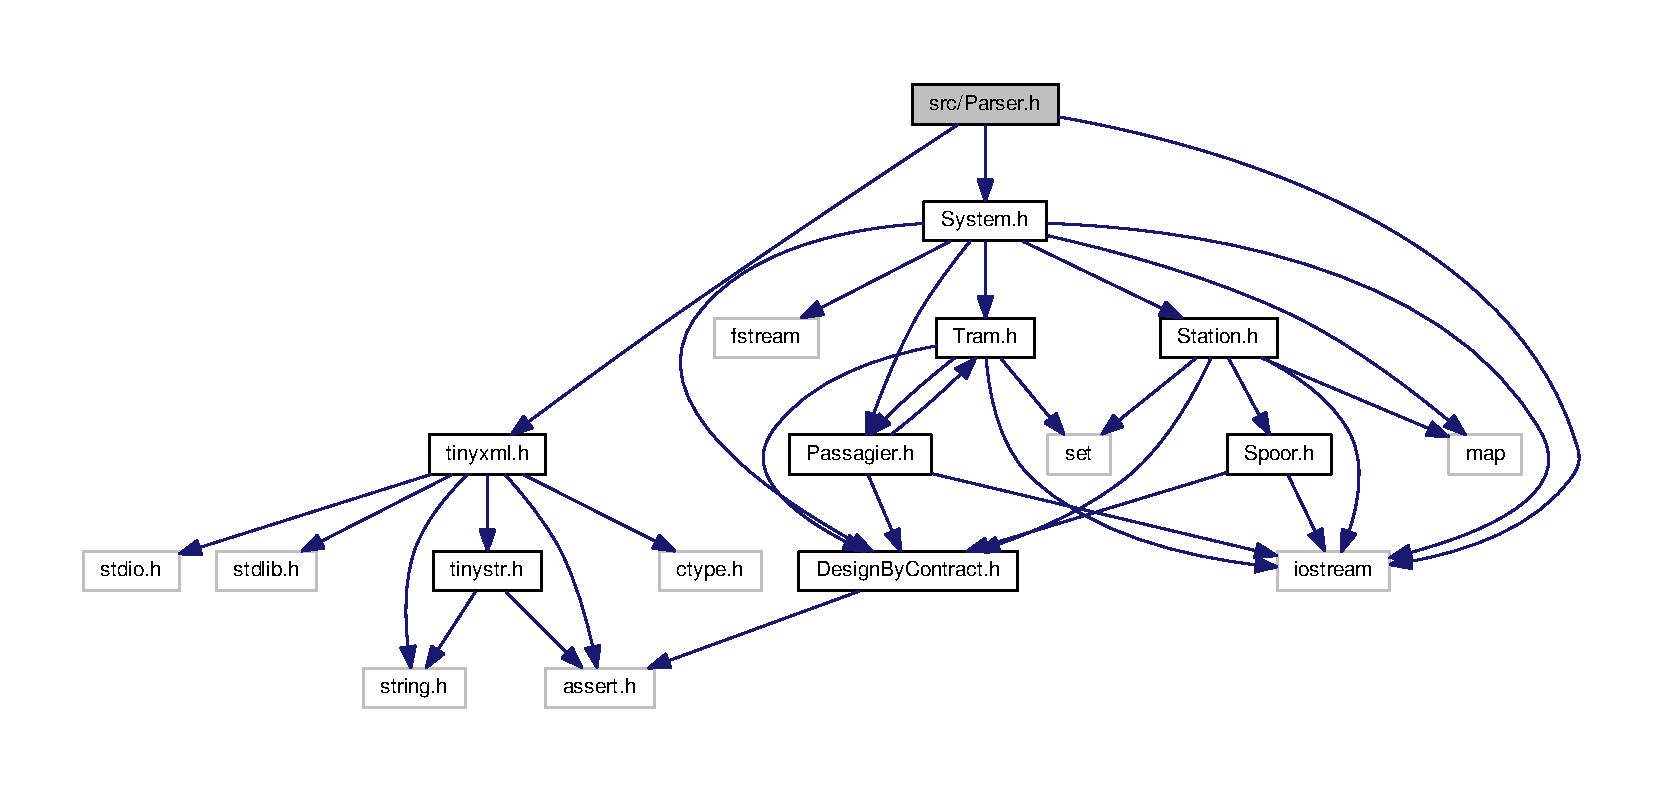
\includegraphics[width=350pt]{Parser_8h__incl}
\end{center}
\end{figure}
\subsection*{Classes}
\begin{DoxyCompactItemize}
\item 
class \hyperlink{classParser}{Parser}
\begin{DoxyCompactList}\small\item\em This Class contains all the functionalities for the \hyperlink{classParser}{Parser} objects. \end{DoxyCompactList}\end{DoxyCompactItemize}


\subsection{Detailed Description}
Header file for the \hyperlink{classParser}{Parser} Class. 


\hypertarget{Passagier_8h}{}\section{src/\+Passagier.h File Reference}
\label{Passagier_8h}\index{src/\+Passagier.\+h@{src/\+Passagier.\+h}}


Header file for the \hyperlink{classPassagier}{Passagier} Class.  


{\ttfamily \#include $<$iostream$>$}\\*
{\ttfamily \#include \char`\"{}Design\+By\+Contract.\+h\char`\"{}}\\*
{\ttfamily \#include \char`\"{}Tram.\+h\char`\"{}}\\*
Include dependency graph for Passagier.\+h\+:
\nopagebreak
\begin{figure}[H]
\begin{center}
\leavevmode
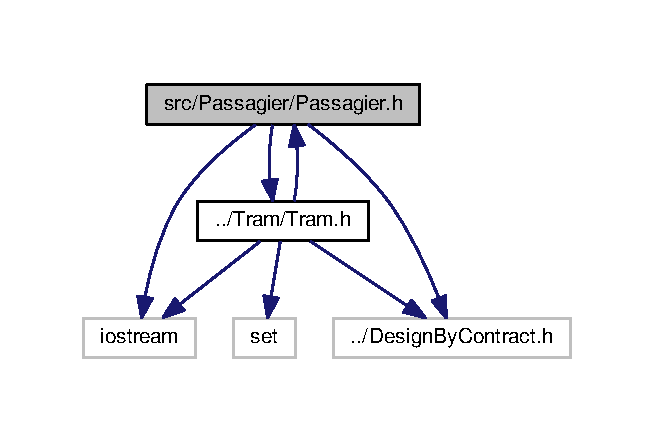
\includegraphics[width=306pt]{Passagier_8h__incl}
\end{center}
\end{figure}
This graph shows which files directly or indirectly include this file\+:
\nopagebreak
\begin{figure}[H]
\begin{center}
\leavevmode
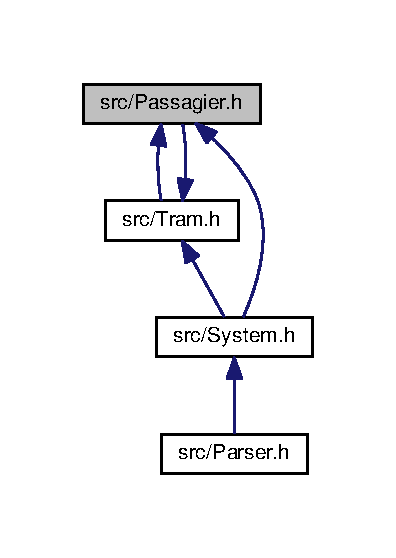
\includegraphics[width=165pt]{Passagier_8h__dep__incl}
\end{center}
\end{figure}
\subsection*{Classes}
\begin{DoxyCompactItemize}
\item 
class \hyperlink{classPassagier}{Passagier}
\begin{DoxyCompactList}\small\item\em This Class contains all the functionalities for the \hyperlink{classPassagier}{Passagier} objects. \end{DoxyCompactList}\end{DoxyCompactItemize}


\subsection{Detailed Description}
Header file for the \hyperlink{classPassagier}{Passagier} Class. 


\hypertarget{Spoor_8h}{}\section{src/\+Spoor/\+Spoor.h File Reference}
\label{Spoor_8h}\index{src/\+Spoor/\+Spoor.\+h@{src/\+Spoor/\+Spoor.\+h}}


Header file for the \hyperlink{classSpoor}{Spoor} Class.  


{\ttfamily \#include $<$iostream$>$}\\*
{\ttfamily \#include \char`\"{}../\+Design\+By\+Contract.\+h\char`\"{}}\\*
Include dependency graph for Spoor.\+h\+:\nopagebreak
\begin{figure}[H]
\begin{center}
\leavevmode
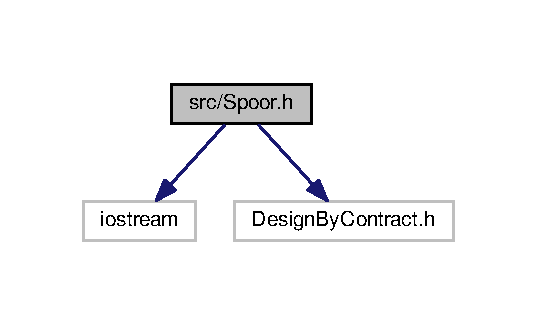
\includegraphics[width=266pt]{Spoor_8h__incl}
\end{center}
\end{figure}
This graph shows which files directly or indirectly include this file\+:\nopagebreak
\begin{figure}[H]
\begin{center}
\leavevmode
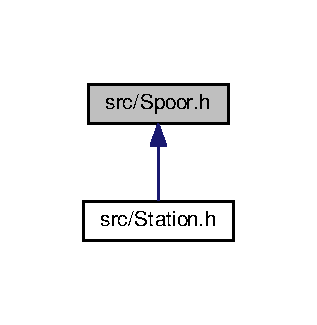
\includegraphics[width=350pt]{Spoor_8h__dep__incl}
\end{center}
\end{figure}
\subsection*{Classes}
\begin{DoxyCompactItemize}
\item 
class \hyperlink{classSpoor}{Spoor}
\begin{DoxyCompactList}\small\item\em This Class contains all the functionalities for the \hyperlink{classSpoor}{Spoor} objects. \end{DoxyCompactList}\end{DoxyCompactItemize}


\subsection{Detailed Description}
Header file for the \hyperlink{classSpoor}{Spoor} Class. 


\hypertarget{Station_8h}{}\section{src/\+Station.h File Reference}
\label{Station_8h}\index{src/\+Station.\+h@{src/\+Station.\+h}}


Header file for the \hyperlink{classStation}{Station} Class.  


{\ttfamily \#include $<$iostream$>$}\\*
{\ttfamily \#include $<$set$>$}\\*
{\ttfamily \#include $<$map$>$}\\*
{\ttfamily \#include \char`\"{}Design\+By\+Contract.\+h\char`\"{}}\\*
{\ttfamily \#include \char`\"{}Spoor.\+h\char`\"{}}\\*
Include dependency graph for Station.\+h\+:\nopagebreak
\begin{figure}[H]
\begin{center}
\leavevmode
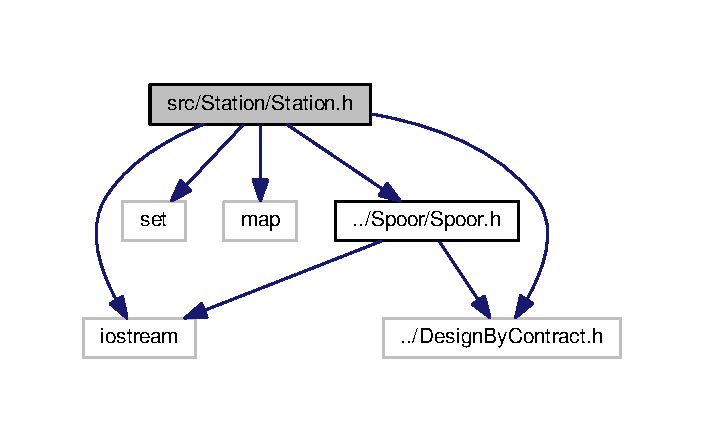
\includegraphics[width=313pt]{Station_8h__incl}
\end{center}
\end{figure}
This graph shows which files directly or indirectly include this file\+:\nopagebreak
\begin{figure}[H]
\begin{center}
\leavevmode
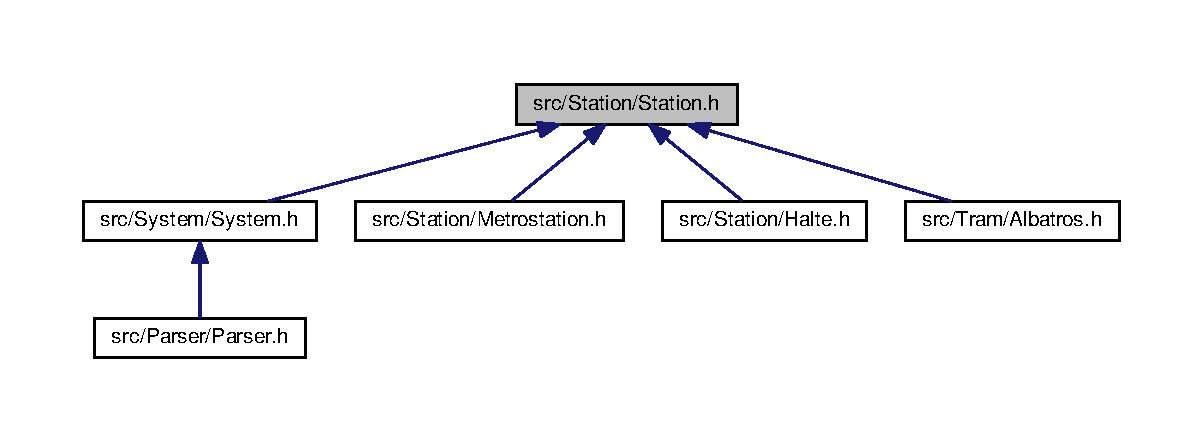
\includegraphics[width=155pt]{Station_8h__dep__incl}
\end{center}
\end{figure}
\subsection*{Classes}
\begin{DoxyCompactItemize}
\item 
class \hyperlink{classStation}{Station}
\begin{DoxyCompactList}\small\item\em This Class contains all the functionalities for the \hyperlink{classStation}{Station} objects. \end{DoxyCompactList}\end{DoxyCompactItemize}


\subsection{Detailed Description}
Header file for the \hyperlink{classStation}{Station} Class. 


\hypertarget{Tram_8h}{}\section{src/\+Tram.h File Reference}
\label{Tram_8h}\index{src/\+Tram.\+h@{src/\+Tram.\+h}}


Header file for the \hyperlink{classTram}{Tram} Class.  


{\ttfamily \#include $<$iostream$>$}\\*
{\ttfamily \#include $<$set$>$}\\*
{\ttfamily \#include \char`\"{}Design\+By\+Contract.\+h\char`\"{}}\\*
{\ttfamily \#include \char`\"{}Passagier.\+h\char`\"{}}\\*
Include dependency graph for Tram.\+h\+:
\nopagebreak
\begin{figure}[H]
\begin{center}
\leavevmode
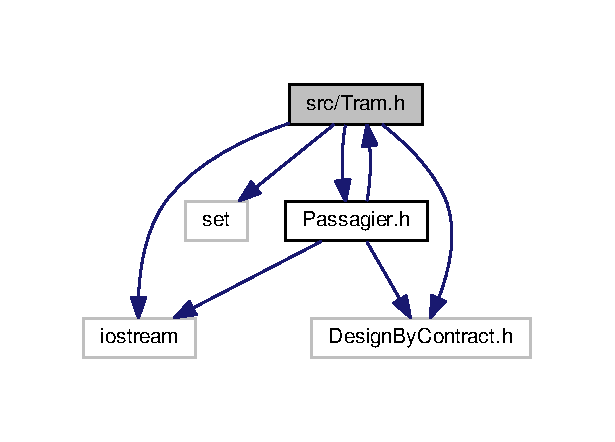
\includegraphics[width=295pt]{Tram_8h__incl}
\end{center}
\end{figure}
This graph shows which files directly or indirectly include this file\+:
\nopagebreak
\begin{figure}[H]
\begin{center}
\leavevmode
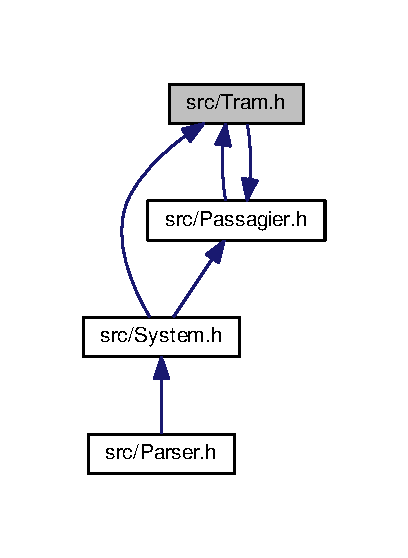
\includegraphics[width=196pt]{Tram_8h__dep__incl}
\end{center}
\end{figure}
\subsection*{Classes}
\begin{DoxyCompactItemize}
\item 
class \hyperlink{classTram}{Tram}
\begin{DoxyCompactList}\small\item\em This Class contains all the functionalities for the \hyperlink{classTram}{Tram} objects. \end{DoxyCompactList}\end{DoxyCompactItemize}


\subsection{Detailed Description}
Header file for the \hyperlink{classTram}{Tram} Class. 


%--- End generated contents ---

% Index
\backmatter
\newpage
\phantomsection
\clearemptydoublepage
\addcontentsline{toc}{chapter}{Index}
\printindex

\end{document}
